\documentclass[conference]{IEEEtran}
\IEEEoverridecommandlockouts
% The preceding line is only needed to identify funding in the first footnote. If that is unneeded, please comment it out.
\usepackage{cite}
\usepackage{amsmath,amssymb,amsfonts}
\usepackage{algorithmic}
\usepackage{graphicx}
\usepackage{textcomp}
\usepackage{xcolor}
\usepackage{hyperref}
\usepackage{amsmath}


\newcommand{\rom}[1]{\uppercase\expandafter{\romannumeral #1\relax}}

\DeclareMathOperator*{\argmin}{arg\,min}

\def\BibTeX{{\rm B\kern-.05em{\sc i\kern-.025em b}\kern-.08em
    T\kern-.1667em\lower.7ex\hbox{E}\kern-.125emX}}
\begin{document}

\title{Assignment 1: a mathematical essay on linear regression\\}


\author{\IEEEauthorblockN{Gautham Govind A}
\IEEEauthorblockA{\textit{Dept. of Electrical Engineering}\\
\textit{Indian Institute of Technology Madras} \\}
\textit{ee19b022@smail.iitm.ac.in}

}

\maketitle

\begin{abstract}
The objective of this assignment is to explore the mathematical formalism behind linear regression and then to use it in a real-life application. In this assignment, as a real-life application, linear regression is used to formally identify the relationship between socioeconomic status and cancer incidence, mortality rates. Linear regression is implemented using Python. The analysis enables us to arrive at the conclusion that the socioeconomic status does indeed have an impact on the cancer incidence. mortality rates. 
\end{abstract}

\begin{IEEEkeywords}
linear regression, python, visualization
\end{IEEEkeywords}

\section{Introduction}

Cancer is one of the most pressing problems faced by society today. While there exists methods to prevent as well as cure cancer, question remains as to whether everyone has easy access to it. It is thus necessary to systematically analyse the impact the socioeconomic status of an individual has on their chance of cancer incidence/ mortality. The goal here is therefore to make use of data to see how cancer incidence/mortality rates of a person is influenced by their income/societal status. 

With the technological advancements we have made, it is now possible to make use of data analytic tools to derive insights from data. By aggregating, cleaning and analysing large amounts of data, it is possible to draw inferences regarding how some parameters may influence others. Linear Regression is one such model which can be used for building linear relationships between variables. The attempt is to make use of Linear Regression to see how various factors affect cancer incidence/mortality of a population.

In this work, we make use of Python for performing the necessary data manipulations. Various libraries in Python are used for cleaning the data, visualizing the data and analyzing the data. Namely, the libraries pandas, seaborn and scikit-learn are extensively used. Jupyter notebook environment is used to easily integrate concise explanation for the code along with the code itself.

After a careful analysis of the available data, and using linear regression, we arrive at the conclusion that the socioeconomic status of an individual does have a significant impact on his chance of cancer incidence/ mortality. More specifically, we find that poverty rate in general has a positive correlation with cancer incidence/ mortality, meaning as poverty rate increases there is a higher chance for cancer incidence/ mortality in that population. We also find that the median income has a negative correlation with cancer incidence/ mortality. Thus, it can be said that low-income groups are at a greater risk of suffering from cancer and it is imperative to address the issue to ensure well being of all members of the society.

Section \rom{2} gives an overview of the various techniques used for data cleaning and an initial exploratory analysis. A lot of insights can be gained just by making qualitative observations from the given data. Section \rom{3} gives a short description of the mathematical formalism behind linear regression. section \rom{4} sates the various results that are obtained by applying linear regression in this particular case. Section \rom{5} gives a summary of the major conclusions drawn from the analysis.

\section{Exploratory Data Analysis}

In this section, we describe the process of data cleaning and visualization.

The given dataset consists of 3134 rows and 25 columns. A brief overview of the dataset is presented in Figure \ref{df_sum}.

\begin{figure}[tbh]
\centering
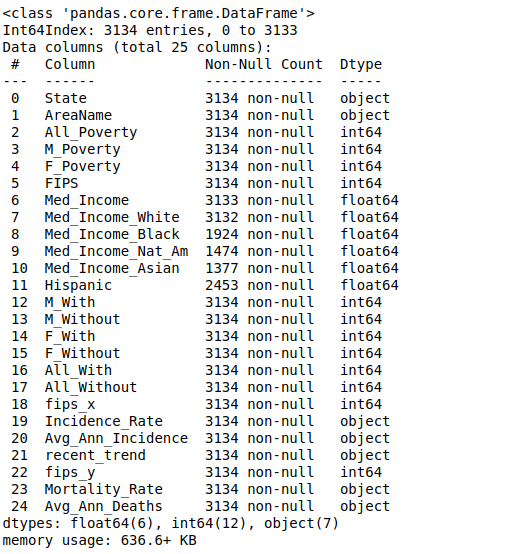
\includegraphics[scale = 0.45]{dataframe_summary.png}
\caption{Summary of the raw dataset}
\label{df_sum}
\end{figure}

Our first task is to weed out columns which are not of relevance. Since our objective is to make inferences for the whole population and not to make inferences for various states/areas separately, discerning between states/areas is unnecessary. This renders columns State, AreaName, FIPS, fips\_x and fips\_y. Hence, we drop these columns.

Next, we observe that the columns Incidence\_Rate, Avg\_Ann\_Incidence, Mortality\_Rate and Avg\_Ann\_Deaths are all marked as having "object" datatype. This is an indication that not all values in these columns are numerical. This will present a problem during mathematical analyses. Hence, it is essential to examine these columns and try to make all values numerical or categorical.

On examination, we find the that there are some non-numerical entries in each of these columns. The type of entry and method adopted to convert it to a numerical value are discussed below:

\begin{itemize}
    \item \textbf{*} - This indicates that the actual value is very low. It seems reasonable to replace these entries using 0. However, this results in the concentration of a lot of values at 0 and severely impedes the performance of regression models. Hence, these rows were removed.
    \item entries ending with \# - This is just an error in formatting. The problem can be resolved by simply removing the \# symbol.
    \item \textbf{\_} and \textbf{\_\_} - These indicate lack of information. Although there are imputation strategies available to deal with such data, we do not apply them here. This is because of two reasons:
    \begin{itemize}
        \item Missing data is present in variables like Incidence\_Rate which is what we would like to predict from other parameters. In this sense, these are like target variables and hence imputation seems non-ideal.
        \item The rows with missing data for these variables accounts for only about 6\% of the total number of rows. Since this is a small fraction, there isn't really a lot of loss of data.
    \end{itemize}
\end{itemize}

After performing all these operations, we are left with a cleaned dataset, whose summary is presented in Figure \ref{mod_df}.

\begin{figure}[tbh]
\centering
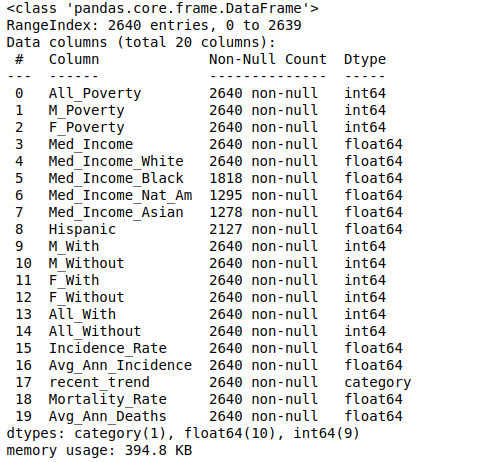
\includegraphics[scale = 0.45]{mod_df.png}
\caption{Summary of the processed dataset}
\label{mod_df}
\end{figure}

At this point, we also make an important observation regarding the variables Incidence\_Rate, Avg\_Ann\_Incidence, Mortality\_Rate and Avg\_Ann\_Deaths. Avg\_Ann quantities represent the \textbf{numbers for the entire population} , whereas Incidence\_Rate and Mortality\_Rate represent the \textbf{numbers normalized using the total population.} Since what is of relevance to us is the normalized rate, we shall be \textbf{considering only Incidence\_Rate and Mortality\_Rate in all further analysis.} 

Our objective is to see the impact of the following two factors on cancer incidence and mortality:
\begin{enumerate}
    \item Economic status
    \item Social status
\end{enumerate}

\subsection{Economic status}

From the available dataset, we make the following observations:

\begin{itemize}
    \item The variables we have with respect to the economic status are the following:
    \begin{itemize}
        \item Number of individuals below poverty line
        \item Median income of individuals
        \item Number of individuals who have health insurance
    \end{itemize}
    \item We expect a \textbf{positive correlation between incidence/mortality rate and poverty rate, whereas a negative correlation between median income and incidence/mortality rate.}
    \item In the case of \textbf{health insurance}, we \textbf{do not expect it to have much impact on the incidence rate} itself, whereas we expect the number of individuals who are insured (normalized with population) to have some \textbf{negative correlation with mortality rate.}
\end{itemize}


On calculating, we observe that \textbf{correlation between All\_Poverty, which is the number of individuals below poverty line, and Incidence\_Rate is -0.027 which is almost 0!} Does this mean there is no correlation between the two? The important fact to note here is that All\_Poverty is the total number of individuals below the poverty line, i.e. it has not been normalized with total population, whereas Incidence\_Rate is already normalized. Hence, it is \textbf{necessary to normalize this quantity as well with respect to total population.}

We can approximate the total population as the sum of all people with health insurance and all people without health insurance. We also calculate male and female population separately. We add these quantities as separate columns and then compute the \textbf{Poverty rate}, which is the number of individuals below poverty lane normalized using population, separately for males and females as well as for the entire population.

After calculating the poverty rates, we calculate the correlation between poverty rate (across all individuals) and incidence rate, mortality rate. We observe correlation values of \textbf{0.259} and \textbf{0.285}, which indicate \textbf{significant positive correlation.} To visualize these observations, we make scatter plots for incidence rate and mortality rate against poverty rate. These plots are presented in Figure \ref{inc_pov} and Figure \ref{mor_pov}.

\begin{figure}[tbh]
\centering
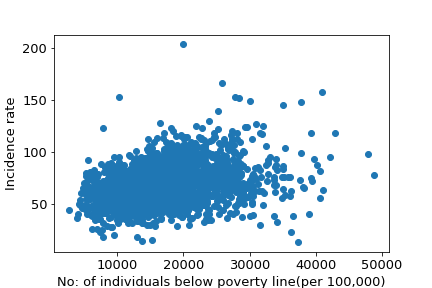
\includegraphics[scale = 0.55]{inc_pov.png}
\caption{Cancer incidence v/s Poverty}
\label{inc_pov}
\end{figure}

\begin{figure}[tbh]
\centering
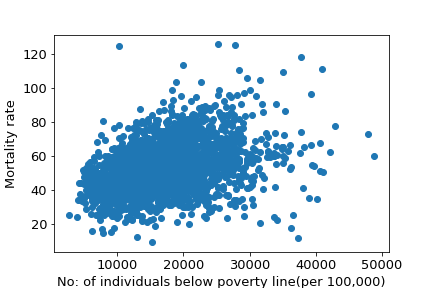
\includegraphics[scale = 0.55]{mor_pov.png}
\caption{Mortality v/s Poverty}
\label{mor_pov}
\end{figure}

From the plots, it is clear that cancer incidence/mortality increases, in general, with increase in poverty.

Next, we observe the relationship between median income and cancer incidence/mortality rate. On calculating, we find that the correlation values are \textbf{-0.256} and \textbf{-0.276} which indicate \textbf{significant negative correlation.} To visualize these observations, we make scatter plots for incidence rate and mortality rate against median income. These plots are presented in Figure \ref{inc_med} and Figure \ref{mor_med}.

\begin{figure}[tbh]
\centering
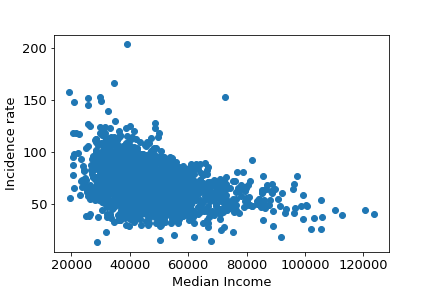
\includegraphics[scale = 0.55]{inc_med.png}
\caption{Cancer incidence v/s Income}
\label{inc_med}
\end{figure}

\begin{figure}[tbh]
\centering
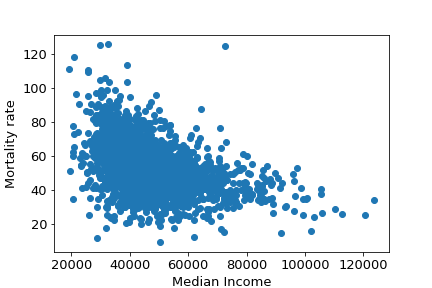
\includegraphics[scale = 0.55]{mor_med.png}
\caption{Mortality v/s Income}
\label{mor_med}
\end{figure}
    
From the plots, it is clear that cancer incidence/mortality decreases, in general, with increase in income.

\textbf{ From the correlation values and plots, it can be qualitatively concluded that as poverty increases/ income decreases, there is a higher chance for cancer incidence/mortality in general.}

We will now consider the impact of having a health insurance on cancer incidence/ mortality. On calculating, we observe correlation values of \textbf{-0.038} and \textbf{-0.124} for incidence and mortality respectively. It seems like there \textbf{isn't any correlation at all between cancer incidence and having a health insurance.} This is to be expected because a health insurance is of use only in the treatment of a disease; not so much for its prevention. Unlike the case of cancer incidence, there seems to be a \textbf{significant negative correlation between having a health insurance and mortality rate.} This is illustrated in Figure \ref{ins_mort}. Again, this is to be expected since having a health insurance provides an incentive to individuals to seek appropriate treatment without considering financial limitations.

\begin{figure}[tbh]
\centering
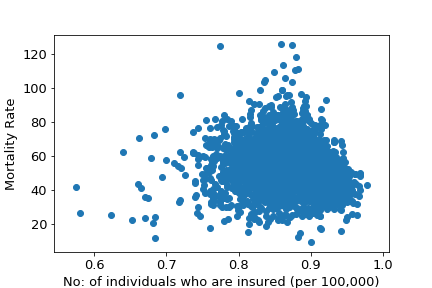
\includegraphics[scale = 0.55]{ins_mort.png}
\caption{Mortality v/s Insurance}
\label{ins_mort}
\end{figure}

\subsection{Social status}

Our target is to associate social status with cancer incidence/ mortality. Towards this, we shall consider the following two broad social classification criterion:

\begin{itemize}
    \item Gender
    \item Ethnicity
\end{itemize}

The major challenge we face in this case is that we \textbf{do not have direct access to incidence/mortality rate for population subsections separately.} For instance, we do not know the separate count of cancer incidence of male individuals and cancer incidence of female individuals. This prohibits any direct comparison. As a result, it is necessary to make an \textbf{indirect comparison} based on the available parameters.

We first consider gender. For gender, we consider the poverty rate for males and females separately. Since we have already concluded from earlier analysis that poverty rate has a positive correlation with both incidence rate and mortality rate, \textbf{if we can conclude that one section has a higher poverty rate in general, we can conclude that this section suffers from higher incidence/mortality as well.} 

To see how the poverty rates of the two sections compare, we make use of a box plot. The box plot is shown in Figure \ref{gend_box}. From the plot, we can \textbf{qualitatively see that females have higher poverty rate, in general.} To make this more quantitative, consider Figure \ref{box_pov_det}. \textbf{Clearly, mean and median of poverty rate of females are higher than males.} Hence, from this, it can be estimated that female population in general has higher poverty rate and \textbf{consequently higher values for cancer incidence and mortality rate.}

\begin{figure}[tbh]
\centering
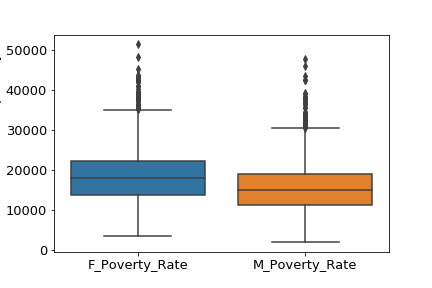
\includegraphics[scale = 0.55]{box_pov.png}
\caption{Gender v/s Poverty}
\label{gend_box}
\end{figure}

\begin{figure}[tbh]
\centering
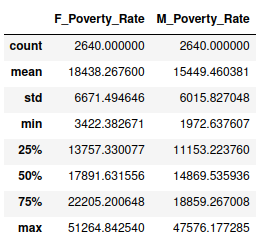
\includegraphics[scale = 0.65]{box_pov_det.png}
\caption{Statistics for poverty distribution}
\label{box_pov_det}
\end{figure}


Next, we explore the relationship between ethnicity and cancer incidence/mortality. In this case, the parameter available to us in median income. As we have seen before, a lower median income would correspond to higher cancer incidence/mortality. To see how the median income varies among different ethnic groups, we again make use of a box plot. The plot is given in Figure \ref{box_ethnic}. It can be seen that the median income of different sections are different, with some sections having higher values and others having lower. A quantitative description is given in Figure \ref{box_ethnic_det}. It can be seen that the mean of the median income follow the following order for ethnic groups:
Asians $>$ Whites $>$ Native Americans $>$ Hispanics $>$ Blacks. Hence, from this, it can be estimated that cancer incidence/mortality rate also follows the same order for ethnic groups.



It must be noted that in all the analysis we have done in this subsection, we have attempted to correlate social status with economic indicators like poverty and income. This approach, though insightful, cannot guarantee a completely accurate analysis, since for this we will need information regarding incidence/mortality rate of each section of the population separately. 

\subsection{Incidence v/s Mortality}

Finally, for the sake of completion, we explore the relationship between cancer incidence and mortality. This is fairly obvious, as we expect a high positive correlation between the two. Visual evidence is presented in Figure \ref{inc_mort}. We observe a correlation of \textbf{0.867} It is also worthwhile to note here that in general as one increases the other also increases with the only exception being the case of insurance rate, which has already been discussed.  

\begin{figure}[tbh]
    \centering
    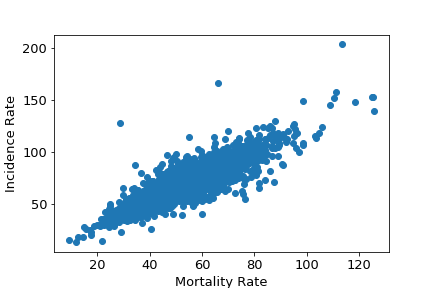
\includegraphics[scale = 0.50]{inc_mort.png}
    \caption{Incidence v/s Mortality}
    \label{inc_mort}
\end{figure}

\begin{figure*}
\centering
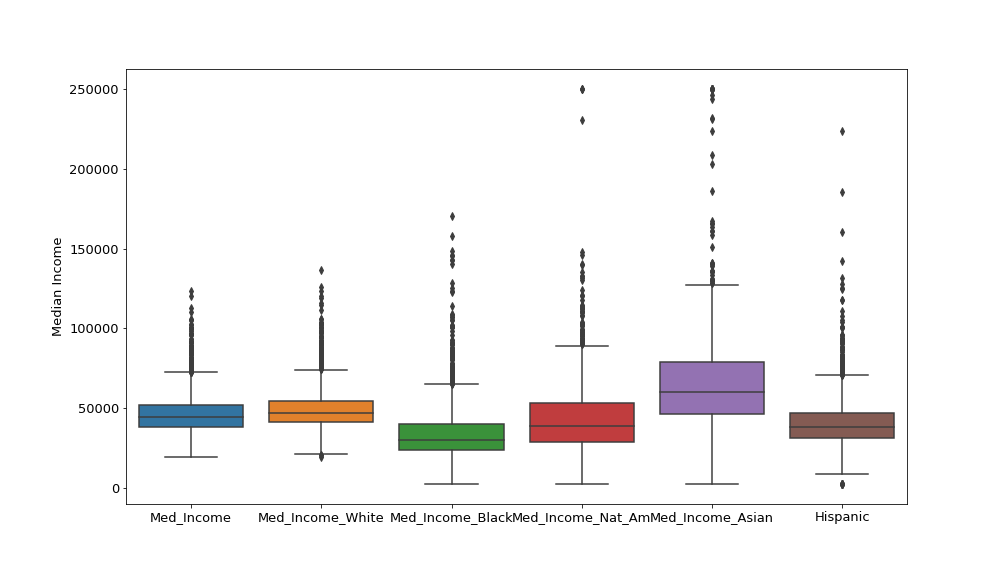
\includegraphics[scale = 0.50]{box_ethnic.png}
\caption{Ethnicity v/s Median income}
\label{box_ethnic}
\end{figure*}

\begin{figure*}
\centering
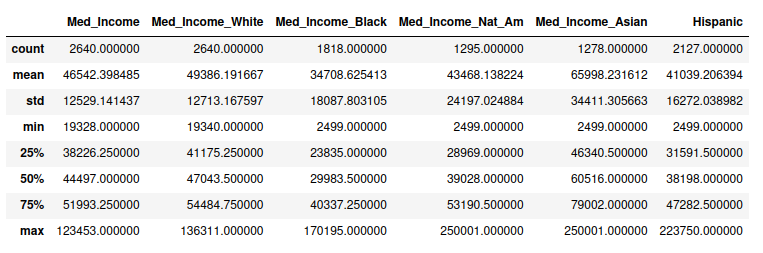
\includegraphics[scale = 0.55]{box_ethnic_det.png}
\caption{Statistics for income distribution}
\label{box_ethnic_det}
\end{figure*}


\section{Model: Linear Regression}

In this section, we will give a brief overview of the mathematical formalism behind the linear regression model. 

Regression is a statistical technique where both the dependent and independent variable takes continuous values and a model is fitted on the explanatory variables. Linear regression is a linear approach for modelling the relationship between a scalar response and one or more explanatory variables. In linear regression, the relationships are modeled using linear predictor functions whose unknown model parameters are estimated from the data.

It must be noted that in general, linear regression is used for creating a linear model of existing data and then using this to predict values for scenarios in which the target variables is unknown. However, in our particular use case, rather than attempting to do this, we will make the model and then use it on the same data; the idea is to see how well the model models the proposed relationship between the variables. A general mathematical description of linear regression is presented below.

Given a data set $  {\displaystyle \{y_{i},\,x_{i1},\ldots ,x_{ip}\}_{i=1}^{n}}  $of n statistical units, a linear regression model assumes that the relationship between the dependent variable y and the p-vector of regressors x is linear. This relationship is modeled through a disturbance term or error variable $\epsilon$ — an unobserved random variable that adds "noise" to the linear relationship between the dependent variable and regressors. Thus the model takes the form:

$$ {\displaystyle y_{i}=\beta _{0}+\beta _{1}x_{i1}+\cdots +\beta _{p}x_{ip}+\varepsilon _{i}=\mathbf {x} _{i}^{\mathsf {T}}{\boldsymbol {\beta }}+\varepsilon _{i},\qquad } $$
for $i=1,\ldots ,n$ and where T denotes the transpose, so that $\mathbf{x_i^T\boldsymbol{\beta}}$ is the inner product between vectors $\mathbf{x_i}$ and $\mathbf{\boldsymbol{\beta}}$. 

Often these n equations are stacked together and written in matrix notation as

    $$ \mathbf {{y} =X{\boldsymbol {\beta }}+{\boldsymbol {\varepsilon }},\,}$$

where

    $$ \mathbf {{y} ={\begin{pmatrix}y_{1}\\y_{2}\\\vdots \\y_{n}\end{pmatrix}},\quad} $$

   $$ {\displaystyle X={\begin{pmatrix}\mathbf {x} _{1}^{\mathsf {T}}\\\mathbf {x} _{2}^{\mathsf {T}}\\\vdots \\\mathbf {x} _{n}^{\mathsf {T}}\end{pmatrix}}={\begin{pmatrix}1&x_{11}&\cdots &x_{1p}\\1&x_{21}&\cdots &x_{2p}\\\vdots &\vdots &\ddots &\vdots \\1&x_{n1}&\cdots &x_{np}\end{pmatrix}},}$$

    $${\displaystyle {\boldsymbol {\beta }}={\begin{pmatrix}\beta _{0}\\\beta _{1}\\\beta _{2}\\\vdots \\\beta _{p}\end{pmatrix}},\quad {\boldsymbol {\varepsilon }}={\begin{pmatrix}\varepsilon _{1}\\\varepsilon _{2}\\\vdots \\\varepsilon _{n}\end{pmatrix}}.}$$

The goal, in general ,is to compute the vector $\boldsymbol{\beta}$ when given $\mathbf{y}$ and $\mathbf{X}$. For the case of simple linear regression, also known as Ordinary Least Squares (OLS), there exists a closed form solution for the following optimization problem, in which we find $\hat{\boldsymbol{\beta}}$ such that:

$$ \hat{\boldsymbol{\beta}} = \argmin_{\boldsymbol{\beta}}{ || \mathbf{X \boldsymbol{\beta} - y} ||^2 }$$

The closed form solution is given by:

$$ \hat{\boldsymbol{\beta}} = \mathbf{(X^TX)^{-1}X^Ty} $$

After computing a solution, it is necessary to have some sort of benchmark to measure the quality of the solution. In our use case, we would like to know how well the chosen parameter represents the target variable. Towards this, we make use of the following two metrics:
\begin{enumerate}
    \item \textbf{Mean Squared Error (MSE)}: MSE is the mean of squares of the error terms, i.e., MSE is given by:
    $$ \textrm{MSE} = \frac{1}{N}\sum_{i=1}^{N}(y_i-\hat{y_i})^2 $$ where $y_i$ is the actual value and $\hat{y_i}$ is the predicted value. Note that this is an absolute metric, meaning the value of MSE cannot be compared across different datasets but can be used for comparison among different models of the same problem.
    \item \textbf{Coefficient of determination ($R^2$)}: $R^2$ is the proportion of the variation in the dependent variable that is predictable from the independent variable(s). It is computed as:
    $$ R^2 = 1 - \frac{\sum_{i = 1}^N(y_i-\hat{y_i})^2}{\sum_{i = 1}^N(y_i-\bar{y_i})^2} $$ where $y_i$ is the actual value, $\hat{y_i}$ is the predicted value and $\bar{y_i}$ is the sample mean given by:
    $$ \bar{y} = \frac{1}{N}\sum_{i = 1}^{N}y_i $$ Unlike MSE, $R^2$ is a relative measure and hence is somewhat data agnostic. Typically, $R^2$ values lies in between 0 and 1, with higher values signifying a better fit.
\end{enumerate}



\section{Modelling }

In this section, we discuss the application the linear regression model to our problem. 

Our primary goal is to identify how cancer incidence and mortality rates are affected by income. More specifically, we would like to see if low-income groups are more prone to cancer and subsequent fatality. The two main parameters we can consider for analysing the income of a particular group are poverty rate and median income.

We employ linear regression keeping cancer incidence rate and mortality as the target variables. We consider the following four models, each taking different input variables:
\begin{enumerate}
    \item Model 1: Poverty rate as the only input variable
    \item Model 2: Median income as the only input variable
    \item Model 3: Both poverty rate and median income as input variables
    \item Model 4: Polynomial features generated from poverty rate and median income as input variables
\end{enumerate}

\subsection{Model 1}

We obtain the plot shown in Figure \ref{m1_inc} for incidence rate and plot shown in Figure \ref{m1_mor} for mortality rate. The values of bench-marking parameters are summarised in Table \ref{tab_m1}.

\begin{figure*}
    \centering
    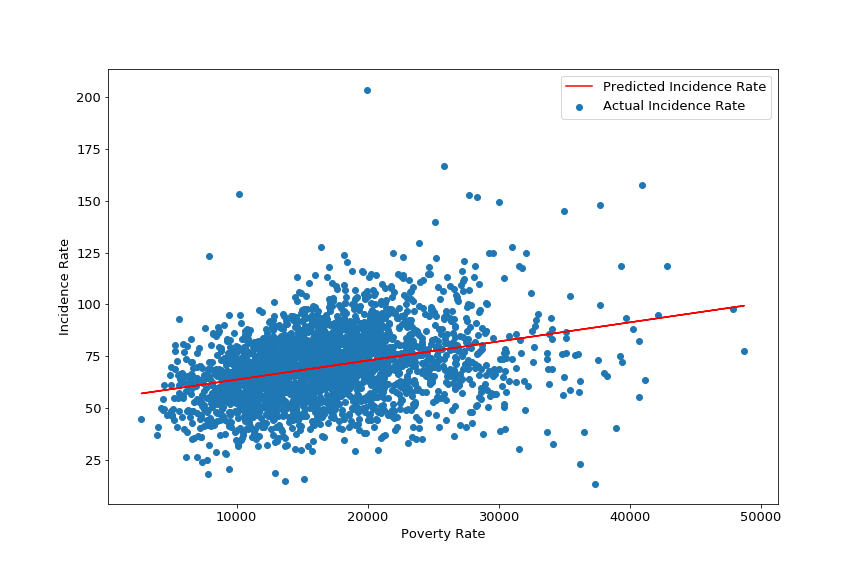
\includegraphics[scale = 0.50]{m1_inc.png}
    \caption{Incidence prediction from poverty rate}
    \label{m1_inc}
\end{figure*}

\begin{figure*}
    \centering
    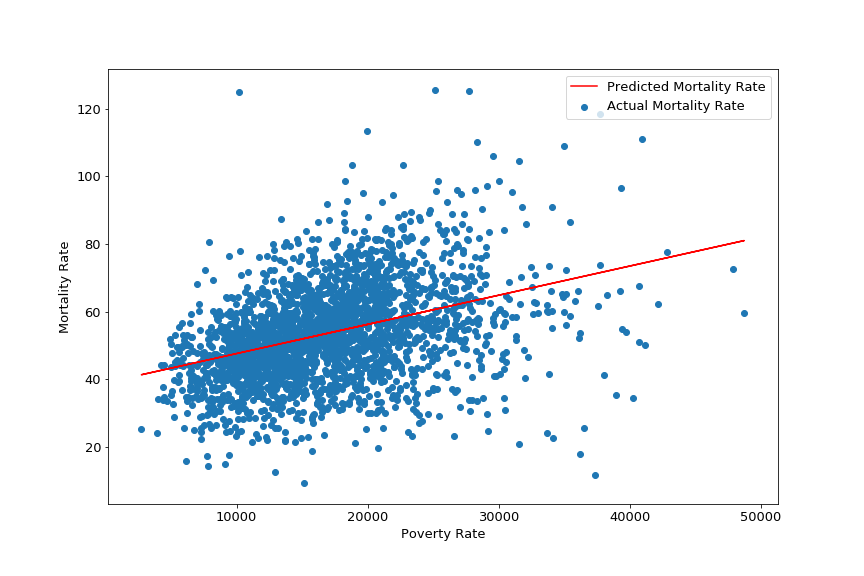
\includegraphics[scale = 0.50]{m1_mor.png}
    \caption{Mortality prediction from poverty rate}
    \label{m1_mor}
\end{figure*}

\begin{figure*}
    \centering
    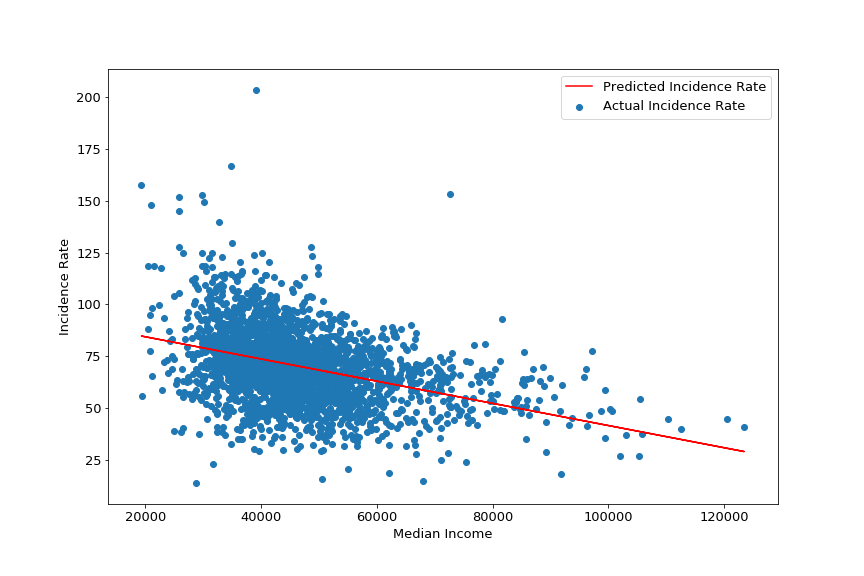
\includegraphics[scale = 0.50]{m2_inc.png}
    \caption{Incidence prediction from median income}
    \label{m2_inc}
\end{figure*}

\begin{figure*}
    \centering
    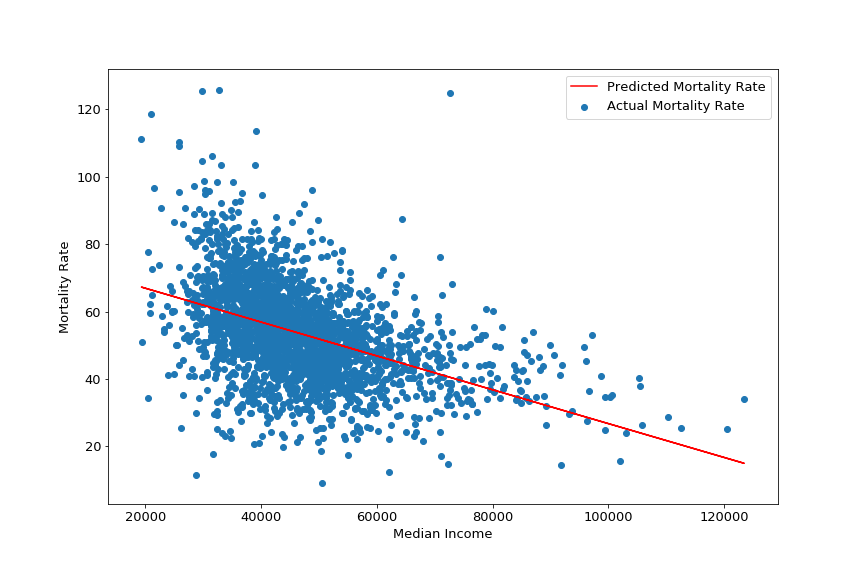
\includegraphics[scale = 0.50]{m2_mor.png}
    \caption{Mortality prediction from median income}
    \label{m2_mor}
\end{figure*}


\begin{table}
\begin{center}

\caption{Benchmarks for Model 1 (Only poverty rate used)}

\begin{tabular}{| c| c| c| }
 \hline
 Type & Incidence Rate& Mortality Rate \\ 
 \hline
 MSE & 279.397 & 169.968 \\  
 \hline
 $R^2$ & 0.107 & 0.147  \\
 \hline

\end{tabular}
 \label{tab_m1}
\end{center}

\end{table}

\subsection{Model 2}

We obtain the plot shown in Figure \ref{m2_inc} for incidence rate and plot shown in Figure \ref{m2_mor} for mortality rate. The values of bench-marking parameters are summarised in Table \ref{tab_m2}.





\begin{table}
\begin{center}

\caption{Benchmarks for Model 2 (Only median income used)}

\begin{tabular}{| c| c| c| }
 \hline
 Type & Incidence Rate& Mortality Rate \\ 
 \hline
 MSE & 267.633 & 159.726 \\  
 \hline
 $R^2$ & 0.144 & 0.198  \\
 \hline

\end{tabular}
 \label{tab_m2}
\end{center}

\end{table}

It can be seen that we obtain \textbf{better fit, in general by using median income instead of poverty rate.} This can be seen in terms of lower MSE values and higher $R^2$ scores.

\subsection{Model 3}

In this case, we give both poverty rate and median income as input paramters. Since, we have two input parameters, it is not possible to visualize the plot in 2D. We can still however obtain the bench-marking parameters. The values of bench-marking parameters are summarised in Table \ref{tab_m3}.

\begin{table}
\begin{center}

\caption{Benchmarks for Model 3 (Income + Poverty)}

\begin{tabular}{| c| c| c| }
 \hline
 Type & Incidence Rate& Mortality Rate \\ 
 \hline
 MSE & 267.032 & 159.186 \\  
 \hline
 $R^2$ & 0.146 & 0.201  \\
 \hline

\end{tabular}
 \label{tab_m3}
\end{center}

\end{table}

It can be seen that we get a better fit than model 2, though only by a marginal amount, again \textbf{signifying that majority of the contribution is from the median income parameter.}

\subsection{Model 4}

In this case, we generate a polynomial of degree 6 from the combination of parameters poverty rate and median income. Again, since we have multiple input parameters, it is not possible to visualize the plot. We can still however obtain the bench-marking parameters. The values of bench-marking parameters are summarised in Table \ref{tab_m4}.

\begin{table}
\begin{center}

\caption{Benchmarks for Model 3 (Income + Poverty)}

\begin{tabular}{| c| c| c| }
 \hline
 Type & Incidence Rate& Mortality Rate \\ 
 \hline
 MSE & 249.674 & 146.292 \\  
 \hline
 $R^2$ & 0.202 & 0.266  \\
 \hline

\end{tabular}
 \label{tab_m4}
\end{center}

\end{table}

It can be seen that we get a \textbf{better fit than model 3, by a significant amount.} This makes sense intuitively because it is not necessary that cancer incidence/mortality is a linear function of poverty rate and median income, but rather can depend on higher powers of these parameters.



\section{Conclusions}

From the four models we have built, it is \textbf{unambiguously clear that cancer incidence and mortality are very much impacted by the socioeconomic status.} By using a mathematical model, it has been formally proved that there exists a \textbf{positive correlation} between poverty rate and cancer incidence/mortality whereas there exists a negative correlation between median income and cancer incidence/mortality. The strength of the correlation has also been \textbf{quantified through bench-marking parameters, namely MSE and $\mathbf{R^2}$.}

It has also been inferred that \textbf{gender and ethnicity play a role in determining the economic status} of an individual as evidenced by the poverty rate and median income distributions. It has also been observed that individuals \textbf{not having a health insurance are at a greater risk of suffering death from cancer as compared to individuals who are insured.}

From the above listed conclusions, it is abundantly clear that \textbf{making health-related policies specifically directed at the low-income sections of the population} is the need of the hour. Focus should be on providing accessible and affordable health insurance as well as treatment to all sections of the population, irrespective of ethnicity and gender.



\section{Avenues for further research}

Although inferences were made regarding how social status affects cancer incidence/mortality, since separate values for cancer incidence/mortality rates for different ethnic/gender sections were not available, direct predictions were not made. Rather, predictions were made indirectly using parameters like median income and poverty. If data can be collected separately for different ethnic/gender groups, a lot more insights can be drawn. Also, there are probably several other parameters which influence cancer incidence/ mortality. A detailed study of these parameters may also be a worthile avenue for further exploration.




\nocite{*} % Print all references regardless of whether they were cited in the poster or not
\bibliographystyle{ieeetr}
\bibliography{sample} % Use the example bibliography file sample.bib


\end{document}
